%*****************************************
\chapter*{Résumé étendu}
\label{chap:resume-etendu}
%*****************************************

\section*{Contexte et motivation}
\label{sec:contexte-et-motivation}

Les solveurs SMT (\emph{Satisfiabilité modulo théories}) \cite{cvc5,verit} se sont imposés comme des outils centraux de la vérification formelle moderne.
Ces solveurs sont utilisés comme des outils pour la démonstration automatique de théorèmes qui intègrent le raisonnement propositionnel enrichies par des théories comme l’arithmétique linéaire, les fonctions non interprétées, ou encore les bit-vectors.
Leur grande efficacité en fait des composants essentiels de nombreux logiciels industriels et académiques, par exemple pour la modélisation et la vérification de systèmes critiques, la vérification de programmes et de matériels, l’analyse statique, ou encore l’intégration dans des assistants de preuve \cite{smtcoq,lean-smt}.

Cependant, cette efficacité s’accompagne d’une question fondamentale de confiance sur les résultats produits.
Les solveurs SMT sont des logiciels complexes, optimisés, et en évolution rapide.
Ils sont en outre souvent écrits en C/C++ pour des raisons de performance, ce qui complique fortement leur vérification formelle et leur formalisation.
Il est donc difficile d’en certifier entièrement l’implémentation, et l’expérience montre que des bogues peuvent conduire à des verdicts incorrects \cite{bugsmt}.
Dans des contextes critiques, où leur résultat entraîne une décision de sûreté, il devient indispensable de renforcer notre confiance dans ces outils.

Une approche prometteuse consiste à certifier non pas l'implémentation du solveur, mais ses résultats, via la technique du \emph{proof logging}.
Cette approche consiste à ce que le solveur produise ainsi une trace de preuve, appelée aussi \emph{certificat}, qui justifie le verdict.
Un outil indépendant, plus simple que le solveur, vérifie ensuite ce certificat.
Cette séparation des rôles est attrayante car la vérification d’une preuve est conceptuellement plus simple et peut s’appuyer sur un noyau de confiance réduit.

\begin{figure}[b]
    \centering
    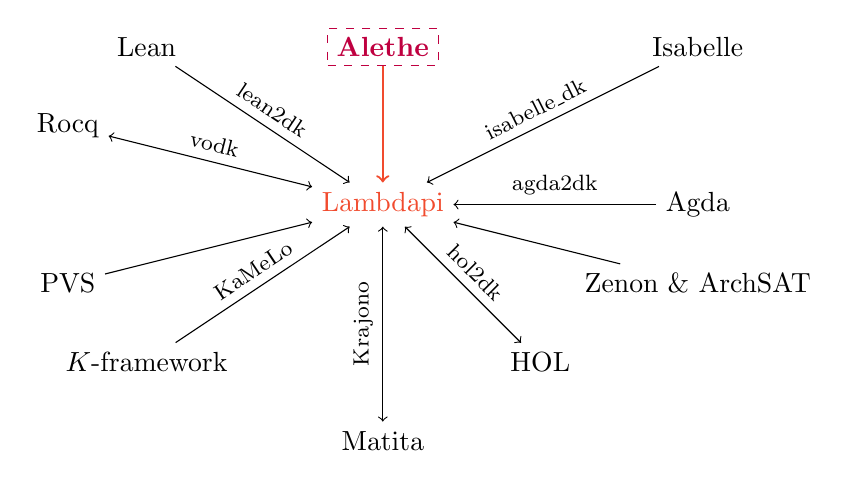
\begin{tikzpicture}
      \path (0,0) node (lp) {\textcolor{RedOrange}{Lambdapi}}
            (-4,1) node (coq) {Rocq}
            (-3,2) node (lean) {Lean}
            (0,2) node [draw, dashed, purple] (smt) {\color{purple}\textbf{Alethe}}
            (4,2) node (isa) {Isabelle}
            (4,0) node (agda) {Agda}
            (-3,-2) node (k) {$\mathbb{K}$-framework}
            (0,-3) node (mat) {Matita}
            (2,-2) node (hol) {HOL}
            (-4,-1) node (pvs) {PVS}
            (4,-1) node (ze) {Zenon \& ArchSAT}
            ;
      \draw[->,RedOrange, thick] (smt) -- (lp) node[midway,sloped,above] {};
      \draw[->] (lean) -- (lp) node[midway,sloped,above] {\footnotesize{lean2dk}};
      \draw[->] (isa) -- (lp) node[midway,sloped,above] {\footnotesize{isabelle\_dk}};
      \draw[->] (agda) -- (lp) node[midway,sloped,above] {\footnotesize{agda2dk}};
      \draw[->] (ze) -- (lp) node[midway,sloped,above] {};
      \draw[<->] (hol) -- (lp) node[midway,sloped,above] {\footnotesize{hol2dk}};
      \draw[<->] (mat) -- (lp) node[midway,sloped,above] {\footnotesize{Krajono}};
      \draw[->] (pvs) -- (lp);
      \draw[->] (k) -- (lp) node[midway,sloped,above] {\footnotesize{KaMeLo}};
      \draw[<->] (coq) -- (lp)  node[midway,sloped,above] {\footnotesize{vodk}};
    \end{tikzpicture}
    \captionsetup{list=no}
    \caption{Lambdapi, un langage assembleur pour les systèmes de preuve.}
    \label{fig:fr-interop-intro}
\end{figure}

Le format Alethe \cite{alethe} a émergé comme un format de preuve standard pour représenter des preuves d’insatisfiabilité SMT.
Alethe repose sur la SMT-LIB \cite{smtlib}. Les preuves sont organisées comme une suite d’étapes, et Alethe propose un catalogue de règles de raisonnement couvrant la résolution, des lemmes de théorie, des simplifications, les quantificateurs et la skolémisation. 
Néanmoins, Alethe ne dispose pas encore d’un vérificateur certifié largement adopté, ce qui limite son rôle comme format d’échange réellement fiable \cite{carcara}.

Cette thèse répond à ce besoin en développant un cadre de \emph{reconstruction} de preuves Alethe dans Lambdapi \cite{lambdapi}.
Lambdapi est un assistant de preuve fondé sur le $\lambda\Pi$-calcul modulo théories, conçu comme un langage pivot pour échanger des preuves entre systèmes.
Comme l’illustre la \Cref{fig:fr-interop-intro}, de nombreux assistants et outils peuvent exporter (ou importer) des preuves via Lambdapi, qui joue alors le rôle de "langage assembleur" pour les systèmes de preuve.
Reconstruire une preuve Alethe dans Lambdapi revient à produire un objet dont la validité est vérifiée par le noyau de Lambdapi, ce qui fournit une garantie forte.
L’objectif est ainsi de rendre les preuves Alethe portables et vérifiables indépendamment du solveur.


\section*{Alethe, preuves SMT et enjeux de vérification}

Le format de traces de preuve Alethe \cite{alethespec} pour les solveurs SMT se compose de deux parties :
un langage de traces, fondé sur SMT-LIB, et une collection de règles de preuve.
Les traces constituent des témoins d’insatisfiabilité d’un ensemble de contraintes.
Elles prennent la forme de séquences $a_1 \dots a_m~t_1 \dots t_n$
où les $a_i$ correspondent aux contraintes du problème SMT initial réfuté,
chaque $t_i$ est une clause inférée à partir des éléments précédents de la séquence,
et $t_n$ est $\bot$ (la clause vide).
Dans la suite, nous désignons le problème SMT-LIB comme le \emph{problème d’entrée}.

\begin{lstlisting}[language=SMT]
(set-logic UF)
(declare-sort U 0)
(declare-fun a () U)
(declare-fun b () U)
(declare-fun p (U) Bool)
(assert (p a))
(assert (= a b))
(assert (not (p b)))
(check-sat)
(get-proof)
\end{lstlisting}

\begin{center}
$\lightning$
\end{center}

\begin{lstlisting}[language=SMT,caption={Un problème SMT et sa preuve Alethe trouvée par cvc5.},label={lst:fr-smtexampleinput-fol},nolol]
(assume a0 (p a))
(assume a1 (= a b))
(assume a2 (not (p b)))
(step t1 (cl (not (= (p a) (p b))) (not (p a)) (p b)) :rule equiv_pos2)
(step t2 (cl (= (p a) (p b))) :rule cong :premises (a1))
(step t3 (cl (p b)) :rule resolution :premises (t1 t2 a0))
(step t4 (cl) :rule resolution :premises (a2 t3))
\end{lstlisting}

L’exemple de la \cref{lst:fr-smtexampleinput-fol} illustre ce principe : à partir du problème d’entrée (ci-dessus), le solveur produit une trace Alethe composée d’étapes \kw{assume} et \kw{step}, aboutissant à la clause vide \kw{(cl)}.

\renewcommand{\eqnhighlightshade}{35}

\begin{equation}
\label{eq:fr-step}
\tag{\textcolor{purple}{1}}
\eqnmarkbox[midpurple]{node2}{i}. \quad \eqnmarkbox[RoyalBlue]{node1}{\Gamma} ~\triangleright~ \eqnmarkbox[Emerald]{node3}{l_1 \dots l_n} \quad (\eqnmarkbox[rxpurple2]{node4}{\mathcal{R}}~\eqnmarkbox[darkpurple]{node5}{p_1 \dots p_m})~\eqnmarkbox[rxpink]{node6}{[a_1 \dots a_r]}
\annotate[yshift=-0.5em]{below, left}{node2}{indèxe}
\annotate[yshift=-0.5em]{below, right}{node1}{contexte}
\annotate[yshift=0.5em]{above, left}{node3}{clause}
\annotate[yshift=-0.5em]{below, right}{node4}{règle}
\annotate[yshift=-0.5em]{below, right}{node5}{prémisses}
\annotate[yshift=-0.5em]{below, right}{node6}{arguments}
\end{equation}

\bigskip

Pour analyser et reconstruire de telles traces, nous décrivons maintenant la structure générale d’une étape Alethe, résumée en \cref{eq:fr-step}.
Une étape est constituée d’un indice \colorbox{midpurple!30}{$i$} $\in \mathbb{I}$, où $\mathbb{I}$ est un ensemble infini dénombrable d’indices (par exemple \kw{a0}, \kw{t1}), et d’une clause de formules \colorbox{Emerald!30}{$l_1, \dots, l_n$} représentant une disjonction $n$-aire.

Les étapes qui ne sont pas des hypothèses sont justifiées par une règle de preuve \colorbox{rxpurple2!30}{$\mathcal{R}$} qui dépend d’un ensemble éventuellement vide de prémisses $\{\colorbox{darkpurple!30}{$p_1 \dots p_m$}\} \subseteq \mathbb{I}$,
ne référant que des étapes antérieures, de sorte que la preuve forme un graphe orienté acyclique.
Une règle peut aussi dépendre d’une liste d’arguments \colorbox{rxpink!30}{$[a_1 \dots a_r]$}, où chaque argument $a_i$ est soit un terme, soit une paire $(x_i, t_i)$, où $x_i$ est une variable et $t_i$ un terme.
L’interprétation des arguments dépend de la règle.

Le contexte \colorbox{RoyalBlue!30}{$\Gamma$} d’une étape est une liste $c_1 \dots c_l$, où chaque élément $c_j$ est soit une variable, soit un couple variable-terme noté $x_j \mapsto t_j$.
Ainsi, les étapes dont le contexte est non vide contiennent des variables $x_j$ qui apparaissent dans \colorbox{Emerald!30}{$l_i$} et seront substituées par les $t_j$.
Les règles de preuve \colorbox{rxpurple2!30}{$\mathcal{R}$} incluent des lemmes de théorie et la règle \texttt{resolution}, qui correspond à l’hyper-résolution sur des clauses du premier ordre au sol.

Ces éléments suffisent pour relire la preuve de la \cref{lst:fr-smtexampleinput-fol}, qui comporte ici sept étapes.
Elle commence par trois étapes \texttt{assume} (\texttt{a0}, \texttt{a1}, \texttt{a2}) qui réaffirment les assertions du problème d’entrée.
Dans la syntaxe concrète, les étapes \texttt{assume} disposent d’une commande dédiée \smtinline{assume}, afin de les distinguer clairement des étapes ordinaires, qui utilisent la commande \smtinline{step}.

L’étape \texttt{t1} introduit une tautologie de la forme $\neg (\varphi_1 \approx \varphi_2) \lor \neg \varphi_1 \lor \varphi_2$, justifiée par la règle \colorbox{rxpurple2!30}{\texttt{equiv\_pos2}}.
L’étape \texttt{t2} établit $p(a) \approx p(b)$ par congruence (règle \colorbox{rxpurple2!30}{\texttt{cong}}) à partir de l’hypothèse \texttt{a1}.
L’étape \texttt{t3} applique ensuite la règle \colorbox{rxpurple2!30}{\texttt{resolution}} aux prémisses \texttt{t1}, \texttt{t2} et \texttt{a0} pour dériver $p(b)$.
Enfin, l’étape \texttt{t4} conclut la preuve en produisant la clause vide $\bot$, concrètement notée \kw{(cl)} dans la \cref{lst:fr-smtexampleinput-fol}.
Remarquons que les contextes \colorbox{RoyalBlue!30}{$\Gamma$} de toutes les étapes sont vides dans cet exemple.

Deux difficultés majeures apparaissent lorsqu’on cherche à vérifier des preuves Alethe.
La première est le caractère parfois \emph{grossier} de certaines règles, qui résument en une étape un calcul ou une simplification non triviale, et peuvent être coûteuses à vérifier naïvement.
La seconde est l’existence de détails de format et de liberté d’impression (par exemple des réordonnancements implicites d’égalités) qui nécessitent une sémantique de vérification soigneuse.

Dans ce travail, l’approche retenue combine deux idées.
D’une part, formaliser et encoder le langage et les règles Alethe dans un cadre fondationnel robuste (Lambdapi).
D’autre part, utiliser une phase d’\emph{élaboration} des traces qui transforme des pas trop ambitieux en séquences plus fines, mieux adaptées à une reconstruction certifiée.

\section*{Lambdapi comme noyau de confiance et langage pivot}

Lambdapi implémente le $\lambda\Pi$-calcul modulo la réécriture, où l’égalité entre termes et types est considérée modulo $\beta$-réduction et un ensemble de règles de réécriture déclarées par l’utilisateur.
Cette capacité à intégrer la réécriture est particulièrement pertinente pour encoder des théories et des calculs de normalisation, tout en conservant une vérification par un noyau de confiance réduit.

Le cadre de cette thèse s’appuie sur une \emph{prélude} logique, suivant un style \emph{judgments-as-types}, dans lequel :
les objets de la logique encodée sont représentés dans un univers \texttt{Set},
les propositions dans un univers \texttt{Prop},
et les preuves comme des termes de type \texttt{Prf A} pour une proposition \texttt{A}.
Cette organisation permet de représenter la logique SMT-LIB (many-sorted first-order logic) et de relier les étapes Alethe à des objets prouvables dans Lambdapi.

Un intérêt central de Lambdapi est également son rôle d’\emph{assembleur} pour systèmes de preuve.
Il sert de pivot permettant, à terme, d’exporter ou d’importer des preuves vers d’autres environnements.
Dans cette perspective, obtenir une reconstruction Lambdapi d’une preuve Alethe rend cette preuve \emph{réutilisable} dans d’autres systèmes, au-delà du solveur qui l’a produite.

\section*{Objectif et contributions de la thèse}

L’objectif général est de construire une chaîne :
\[
\text{preuve Alethe (solveur)} \;\longrightarrow\;
\text{élaboration (trace plus fine)} \;\longrightarrow\;
\text{traduction en Lambdapi} \;\longrightarrow\;
\text{vérification par le noyau}.
\]
Cette chaîne fournit une garantie indépendante de la correction du solveur, sous réserve de la confiance accordée au noyau de Lambdapi.

Les contributions principales sont les suivantes.
Premièrement, une \emph{encodage modulaire} de la logique SMT-LIB et des objets Alethe (termes, formules, clauses, substitutions, sous-preuves) dans Lambdapi.
Deuxièmement, une méthode de \emph{reconstruction} couvrant un ensemble substantiel de règles Alethe, incluant la résolution, des simplifications, des quantificateurs, et des fragments d’arithmétique linéaire.
Troisièmement, l’introduction de techniques de \emph{preuve par réflexion} pour rendre la vérification de calculs arithmétiques efficace et robuste.
Quatrièmement, une étude de \emph{correction} de la traduction, assurant que les certificats reconstruits préservent le sens sémantique des preuves SMT.
Enfin, une \emph{évaluation expérimentale} sur des benchmarks issus de SMT-LIB et sur des obligations de preuve TLA+ (via TLAPS), avec des optimisations de performance comme la traduction et la vérification parallèles.

\section*{Encodage de la logique SMT et des clauses}

La logique SMT-LIB est une logique du premier ordre à plusieurs sortes.
Un point clé de l’encodage consiste à représenter les sortes et les termes de manière fidèle tout en restant maniable dans Lambdapi.
Les connecteurs logiques sont introduits de façon constructive, avec une représentation des preuves via \texttt{Prf}.
Les quantificateurs sont encodés en quantifiant sur des éléments de \texttt{Set} et en réifiant la dépendance par \texttt{El}.
Cette approche permet d’exprimer des formules proches de SMT-LIB tout en conservant un contrôle explicite sur les preuves.

Alethe raisonne sur des \emph{clauses} et non directement sur des formules arbitraires.
La thèse introduit donc une représentation des clauses adaptée à la reconstruction.
Elle doit gérer :
la disjonction n-aire,
les littéraux positifs et négatifs,
et les conventions de format (par exemple la clause vide représentant la contradiction).
Cet encodage sert ensuite de base aux règles de reconstruction, notamment la résolution.

\section*{Reconstruction des preuves du premier ordre}

Pour les règles propositionnelles et du premier ordre, la reconstruction suit une stratégie en deux niveaux.
D’abord, les règles \emph{tautologiques} (introductions d’identités, transformations logiques simples) sont traitées par des preuves relativement directes dans Lambdapi.
Ensuite, les règles de \emph{déduction} (résolution, chaînages) sont reconstruites par des lemmes génériques sur les clauses, permettant de factoriser les preuves et de réduire la duplication.

Les quantificateurs et la skolemisation constituent une partie délicate.
Les traces Alethe comportent des règles comme l’instanciation universelle et des pas liés au traitement des variables liées.
La thèse formalise ces mécanismes en combinant :
une représentation explicite des substitutions,
des lemmes de compatibilité avec la structure des termes,
et des constructions de preuve qui respectent les contraintes de capture et d’$\alpha$-équivalence.

Les sous-preuves Alethe (\emph{subproofs}) sont également reconstruites.
Elles correspondent à des contextes temporaires d’hypothèses, dont la décharge doit être représentée explicitement dans Lambdapi.
La stratégie consiste à refléter la discipline Alethe (hypothèses locales, puis règle de décharge) par des constructions d’implication et de clauses adaptées.

\section*{Reconstruction de l’arithmétique linéaire par réflexion}

L’arithmétique linéaire est un domaine où les solveurs SMT utilisent des algorithmes sophistiqués (simplex, branch-and-bound, coupes, etc.).
Les preuves Alethe contiennent souvent des étapes qui encapsulent des calculs arithmétiques ou des normalisations.
Les vérifier pas à pas au niveau logique serait trop coûteux.

La thèse adopte alors une approche par \emph{réflexion}.
L’idée est de représenter les expressions arithmétiques sous une forme \emph{réifiée} (une syntaxe interne),
de définir une procédure de normalisation sur ces objets,
puis de prouver dans Lambdapi un théorème de correction disant que la normalisation préserve la sémantique.
Ainsi, au lieu de reconstruire un raisonnement arithmétique long, on reconstruit la preuve que la procédure de normalisation est correcte, puis on l’applique.

Deux niveaux de normalisation sont étudiés.
Une normalisation \emph{interne} vise à mettre les polynômes sous une forme canonique en utilisant des propriétés comme l’associativité et la commutativité.
Une normalisation \emph{externe} traite des réécritures plus globales et des schémas de comparaison et d’assemblage de contraintes.
Ces techniques permettent de traiter efficacement de nombreux certificats d’arithmétique linéaire.

\section*{Élaboration des traces : affiner pour mieux vérifier}

Une contribution essentielle est la phase d’élaboration.
Dans l’écosystème étudié, des outils comme Carcara et RARE transforment les preuves Alethe produites par les solveurs en preuves plus adaptées à la reconstruction.
L’élaboration peut notamment :
éliminer des pas redondants,
expliciter des réordonnancements implicites,
décomposer des règles trop grossières en sous-étapes plus élémentaires,
ou remplacer des simplifications complexes par des séquences compatibles avec les bibliothèques de preuve disponibles.

Cette étape d’élaboration joue un rôle analogue à une phase de compilation.
Elle permet de passer d’une preuve « orientée solveur » à une preuve « orientée vérification ».
Le gain est double :
on augmente le taux de reconstruction réussie,
et on améliore les performances de vérification en Lambdapi en évitant des règles difficiles.

\section*{Correction de la traduction}

La reconstruction n’est utile que si elle est correcte.
La thèse établit donc un argument de correction montrant que la traduction préserve l’entaillement sémantique.
Intuitivement, si une étape Alethe est valide au sens de la sémantique Alethe/SMT-LIB, alors la preuve construite dans Lambdapi démontre une proposition correspondante dans l’encodage.

Cet argument mobilise :
la correspondance entre clauses Alethe et formules encodées,
la correction des lemmes de reconstruction pour chaque règle supportée,
et, pour la partie arithmétique, la correction des procédures réflexives de normalisation.

Le résultat est une chaîne de confiance claire :
la validité finale repose sur le noyau de Lambdapi et sur les hypothèses explicites de l’encodage (notamment la correction des définitions et des lemmes de base).

\section*{Évaluation expérimentale et étude de cas TLAPS}

La thèse évalue la méthode sur des ensembles de benchmarks.
L’objectif est de mesurer :
le taux de reconstruction (succès/échec/timeouts),
les temps d’élaboration, de traduction et de vérification,
et l’impact de diverses optimisations.

Une attention particulière est portée à la scalabilité.
Les preuves SMT peuvent être volumineuses, et la reconstruction doit rester praticable.
La thèse étudie ainsi des optimisations comme la parallélisation de la traduction et de la vérification,
ainsi que des stratégies de découpage et de gestion mémoire.

En outre, une étude de cas importante concerne des obligations de preuve issues de TLA+,
via TLAPS, et résolues par un solveur SMT produisant des traces Alethe.
La reconstruction dans Lambdapi illustre alors une chaîne complète de vérification,
depuis un environnement de spécification (TLA+) jusqu’à une preuve certifiée dans un assistant fondationnel,
en montrant la pertinence de l’approche pour des preuves issues d’outils de vérification concrets.

\section*{Conclusion et perspectives}

Cette thèse propose une contribution vers un écosystème SMT plus fiable et plus interopérable.
En reconstruisant des preuves Alethe dans Lambdapi, on obtient des certificats vérifiables indépendamment,
et potentiellement exportables vers d’autres assistants.
L’approche combine :
un encodage modulaire de la logique SMT,
des techniques de reconstruction génériques pour le premier ordre,
et des méthodes réflexives efficaces pour l’arithmétique linéaire,
le tout soutenu par une phase d’élaboration qui rapproche les traces du format attendu par le vérificateur.

Plusieurs perspectives s’ouvrent naturellement.
Étendre la couverture à d’autres théories importantes, comme les bit-vectors ou certaines formes de quantificateurs plus riches, renforcerait encore l’universalité du cadre.
Améliorer l’élaboration pour traiter davantage de variations de solveurs et de versions du format,
et optimiser la performance de la reconstruction sur des preuves très grandes,
sont également des axes pratiques majeurs.
Enfin, approfondir l’intégration avec d’autres assistants (export vers Rocq, Isabelle/HOL, Lean) contribuerait à faire d’Alethe un véritable format d’échange de preuves,
au service d’une vérification formelle plus transparente et plus digne de confiance.

\setcounter{figure}{0}
\setcounter{equation}{0}
\setcounter{table}{0}
\setcounter{lstlisting}{0}
